% Chapter 1

\chapter{Introduction} % Main chapter title

\label{1.} % For referencing the chapter elsewhere, use \ref{Chapter1} 

%----------------------------------------------------------------------------------------

% Define some commands to keep the formatting separated from the content 
\newcommand{\keyword}[1]{\textbf{#1}}
\newcommand{\tabhead}[1]{\textbf{#1}}
\newcommand{\code}[1]{\texttt{#1}}
\newcommand{\file}[1]{\texttt{\bfseries#1}}
\newcommand{\option}[1]{\texttt{\itshape#1}}


%----------------------------------------------------------------------------------------


With ever more sensors in use and ever more gadgets and smart devices like smartphones, smartwatches or even fridges, the amount of available data steadily increases. Simultaneously, the possibilities to use the data to draw conclusions increases. Recently, data is used not only to draw conclusions but also to predict behavior such as failure of sensor or a heart attack. \textcolor{red}{Examples mit Quellen} These events typically occur very rarely. However, when the number of instances of each class is approximately equal, most machine learning algorithms function best. Problems occur when the number of instances of one class greatly exceeds the number of instances of the other. This issue is very popular in practice, and it can be observed in a variety of fields such as fraud detection, medical diagnosis, oil spillage detection, facial recognition, and so on. The task of identifying the rare item, event or observation is often referred to as anomaly detection. Typically, the anomalous item translates to problems such as bank fraud or medical problems. Often, the anomaly does not adhere to the common statistical definition of an outlier. Therefore, many outlier detection methods (in particular unsupervised methods) fail on such data. 

A special disciplin in anomaly detection is to find the anomaly in a time series. The anomaly detection problem for time series is usually formulated as finding outlier data points relative to some standard or usual signal. Time series anomaly detection plays a critical role in automated monitoring systems. It is an increasingly important
topic today, because of its wider application in the context of the Internet of Things (IoT), especially in industrial environments. The most popular techniques to find the anomalies are:

\begin{itemize}
	\item Statistical Methods
	\item Support Vector Machines
	\item Clustering 
	\item Density-based Techniques
	\item Neural Networks 
\end{itemize}

\section{Definitions}

\subsection{Univariate, Bivariate and Multivariate Data}
Time series data comes in different forms. It is distinguished between univariate, bivariate and multivariate data. Univariate involves the analysis of a single variable while bivariate and multivariate analysis examines two or more variables.

\subsubsection{Univariate Data}
There is only one variable in this type of data. Because the information only deals with one variable that changes, univariate data analysis is the simplest type of analysis. It is not concerned with causes or relationships, and the primary goal of the analysis is to describe the data and identify patterns.

\subsubsection{Bivariate Data}
This type of data involves two different variables. This type of data analysis is concerned with causes and relationships, and the goal is to determine the relationship between the two variables.

\subsubsection{Multivariate Data}
Multivariate data is defined as data that contains three or more variables. It's similar to bivariate, but there are more dependent variables. The methods for analyzing this data are determined by the objectives to be met. Regression analysis, path analysis, factor analysis, and multivariate analysis of variance are some of the techniques.

\subsection{Neuron}

\subsection{Layer}



\section{Background}

\subsection{Neural Networks for Anomaly Detection}


expain neural networks\\

Out of the three most popular neural network architectures, convolutional neural networks (CNN), recurrent neural networks (RNN) and deep neural networks (DNN), only RNN are typically used for anomaly detection in time series. RNNs have built-in memory and are therefore able to anticipate the next value in a time series based on current and past data. Classic or vanilla RNNs can theoretically keep track of arbitrary long-term dependencies in input sequences. There, however, exists a computatinal issue: when using back-propagation to train a vanilla RNN, the back-propagated gradients can "vanish" or "explode" due to the computations involved in the process, which use finite-precision numbers. Because LSTM units allow gradients to flow unchanged, RNNs using LSTM unit or Gated Recurrent units (GRU) partially solve the vanishing gradient problem and therefore drastically improve accuracy.

Especially to mention in this context are LSTM (Long-Short Term Memory) and GRU (Gated Recurrent Units). Both achieved outstanding performance when used for tasks such as unsegmented, connected handwriting recognition, speech recognition and anomaly detection in network traffic or IDSs (intrusion detection systems). \textcolor{red}{QUELLEN von Wikipedia}//



\subsubsection{LSTM}
LSTM was first proposed in 1997 by Schmidhuber and Hochreiter. The initial version to the LSTM unit consisted of a cells, input and output gates. In 1999, the LSTM architecture was improved by introducing a forget gate and therefore allowing the LSTM to reset its own state. LSTM is used in a supervised training approach, that means it tries to predict a predefined state taking the past and the current state. If the predicted state differs from the expected state, the weights of the different gates are adjusted using an optimizer algorithm such as gradient descent. Figure \ref{fig:LSTM} shows how the gates and the cell are arranged. The cell represents the memory of the LSTM. In simple words, the LSTM works as follows to predict a new value: 

\begin{enumerate}
	\item Forget Gate: Obsolete information is removed from the cell state.
	\item Input Gate: New information is added to the cell state
	\item Output Gate: The new information and the cell state are added to make the new prediction.
	\item The new cell state is propagated to the next LSTM unit  
\end{enumerate}
     
\begin{figure}
	\centering
	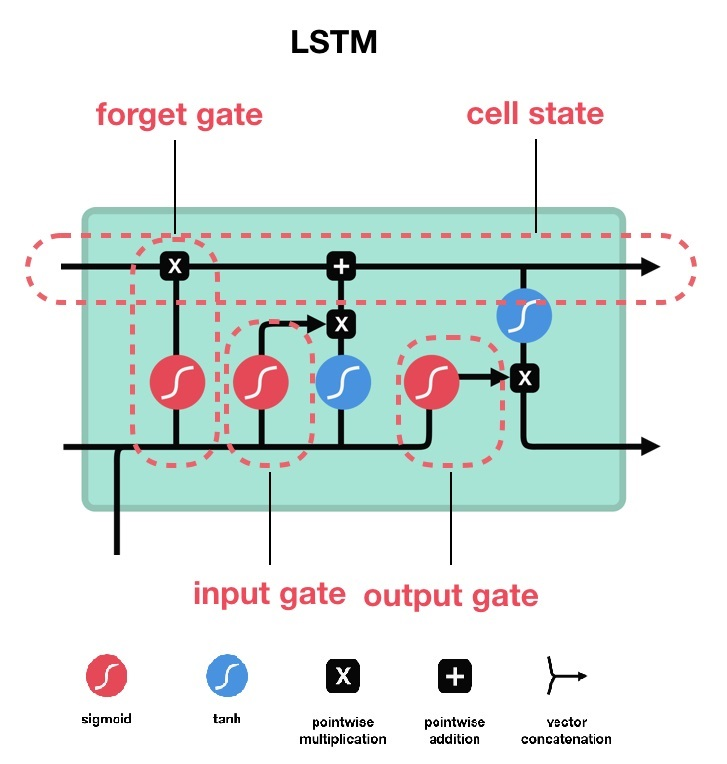
\includegraphics[scale=0.5]{Figures/LSTM}
	\decoRule
	\caption[LSTM]{Gates and Cell of LSTM}
	\label{fig:LSTM}
\end{figure}


\subsubsection{GRU}
% maybe not necessary

\subsubsection{CNN}
In contrast to RNNs Convolutional Neural Networks are generally for image classification. CNNs work as feature extractors and are able to recognize patterns. CNNs use layers that are not fully connected, to reduce complexity. In a CNN, a set number of neurons forms a filter. These filters or kernels are the actual feature extractors. A filter may represent a line or pattern.

To detect whether, a feature is occurent in a picture, the filter is gradually moved over the picuter in so called strides.  \\ 

use animation to show the stride and filter\\

In 2019, Wen and Keys proposed to use CNN also for anomaly detection in time series since it shares many common aspects with image segmentation. A univariate time series is therefore viewed as a one-dimensional image.\\ 

- refer to filters that CNNs use


\section{Problem Statement}

\begin{itemize}
	\item  What is the problem?
	\item Why is it a problem?
	\item What facets are there to it?
	\item What has been done to address it before, if anything, and why is
	that not satisfactory?
	\item Clearly state what is the gap -- Are CNN really useful?
\end{itemize}
Section about transfer learning\\

The main goal of this research project is to clarify whether CNNs are really useful and propose an advantage over RNNs when applied on time series data for anomaly detection.


\section{Thesis Statement}

Convolutional Neural Networks are superior to Recurrent Neural Networks when looking for anom

Problems:
- mention the comparison!!
 - RNN takes long to train!
 - Design changes for multivariate data
 - Design changes for time series data
 - How can the different architectures be compared
 - what influence has transfer learning on the two approaches
 - limitations?\\

Defining a ground truth is one of the most difficult aspects of time series anomaly detection. Determining when anomalous behavior begins and ends in time series is a difficult task, as even human experts are likely to disagree in their assessments. Furthermore, there is the question of what constitutes a useful detection when detecting anomalies in time series.
In the past, RNN have successfully been used for anomaly detection. Therefore, designs for various use cases are well researched. RNN are the best suited for task, however, take a long time to train due to the complexity of how a single unit is designed. In comparison CNN are not as complex. However, CNNs are generally used for image recognition and were only very recently used for anomaly detection in time series. It is therefore mostly unknown what designs are applicable for succesful anomaly detection in time series data. 

%is this true?
While RNN are able to deal with multivariate data by design, a classical CNN requires design changes to be able to deal with multivariate data. 

Further, a CNN is not capable to analyze streaming data so it relies on segmentation of the data. These data segments are called snapshots. In order to not miss any data points, the frequency of taking these snapshots should be at least as high as the length of snapshot so that every time point is evaluated by the model at least once. However, for better performance it might prove beneficial to use a higher frequency which means every point is evaluated various times by the model \parencite{wen2019time}. The length and frequency of the snapshot are only two of many parameters to be chosen for both architecture types. Other important parameters, next to the frequency which are to be determined are the number of epochs (iterations) or the training time. These parameter 
\\alies in time series data regarding training and complexity.


\subsection{Subquestions}

\begin{itemize}
	\item How does a CNN for univariate and multivariate data need to be designed for succesful anomaly detection in time series data?
	\item What advantages and disadvantages arise when using a CNN compared to a RNN for anomaly detection in univariate and multivariate time series?
	\item Which settings are crucial for a fair performance comparison between RNN and CNN? 
	\item Optional: How does transfer learning affect the performance of CNN compared to RNN in anomaly detection in time series?
\end{itemize}



 
\subsection{Research Objectives}

always start with a verb ... to test, to determine

refer to the subquestions

\subsection{Limitations}

-- not looking at combinations of CNN and RNN

\subsection{Significance}

-- why is my work relevant

\subsection{Chapter Overview}


%----------------------------------------------------------------------------------------
